\chapter{Реализация}
\label{chapter_implementation}

\section{Введение} \label{sect_impl_introduction}

При переходе от теории к практике становится важным уделять большее внимание эффективности применяемых алгоритмов.
В этом разделе будут описаны оптимизации теоретически разработанных алгоритмов, которые позволяют применять их для реальных программных систем. 

Первая такая оптимизация касается хранения достижимых состояний. В теории для определения состояния гонки необходимо было для каждой пары достигнутых состояний проверить наличие обращения к одинаковой разделяемой памяти. Такой простой алгоритм был совершенно не эффективен. Количество различных состояний может превышать десять миллионов. Поэтому необходимы очень эффективные алгоритмы хранения и поиска пары состояний образующих состояние гонки. В подразделе~\ref{sect_impl_storage} будут описаны соответствующие оптимизации.

Процесс уточнения построенной абстракции может занимать достаточно много времени даже при решении задачи достижимости. При поиске состояний гонки может быть необходимо уточнить абстракцию сразу для нескольких обнаруженных состояний гонки. Уточнение абстракции последовательно становится очень неэффективным. В подразделе~\ref{sect_impl_refinement} описан процесс уточнения абстракции и применяемые оптимизации.

Важной задачей, на которую многие академические инструменты не обращают внимания, является понятное и наглядное представление результатов верификации. Это особенно важно для описания ошибок, связанных с параллельным выполнением нескольких потоков, так как при этом не достаточно указать только строку или переменную, в которой возможно наличие ошибки. Необходимо представить полную трассу выполнения потоков, выделив некоторые важные события, например, создание потоков, захват примитивов синхронизации и одновременные доступы к разделяемой памяти. В подразделе~\ref{sect_impl_visualiztion} будут описан алгоритм печати трассы.

\section{Обзор инструмента} \label{sect_impl_storage}

Описание анализов

LockCPA

ThreadCPA

PredicateCPA
%Тоже сделать частью Usage?

UsageCPA

BAMCPA

Картинка

Пример работы 

\section{Оптимизации хранения данных} \label{sect_impl_storage}

\subsection{Block Abstraction Memoization} \label{subsect_impl_bam}

В процессе анализа используется оптимизация, использующая абстрактные блоки (англ. Block Abstraction Memoization, BAM). 
Эта оптимизация позволяется переиспользовать результаты, полученные в процессе анализа.
Например, если функция уже была проанализирована, и та же самая функция вызывается второй раз, анализировать ее заново не обязательно, если контекст ее вызова тот же самый.
Абстрактными блоками, на границах которых производится кэширование результатов, могут быть как функции, так и тела циклов. 

Каждый анализ описывает специальный механизм выделения существенной части из своего абстрактного состояния. Это операция reduce. 
При входе анализом в новый абстрактный блок выполняется операция reduce. Полученное "уменьшенное" состояние ищется в кэше.
В случае, если результат уже присутствует к кэше, то есть анализ для данного состояния уже проводился ранее, выполняется операция expand, которая на основе полного исходного состояния и неполного результирующего состояния строит полное результирующее состояние. 
Если же фиксируется промах в кэше, это значит, что нужно провести анализ и сохранить его результат. 

\subsection{Идентификаторы доступа к переменным} \label{subsect_impl_identifiers}


\subsection{Накопление результатов в процессе анализа} \label{subsect_impl_storage}

Для каждого доступа к переменной формируется специальная структура данных, содержащая информацию об этом доступе. 
Будем использовать обозначение $Usage$ для этой структуры данных.

\begin{align}
& Usage = (line, access, state, states, id) \nonumber \\ 
& line \in \mathbb{N}, access \in \{READ, WRITE\}, state \in E, states \in 2^E, id \in ID \nonumber
\end{align}

Здесь $line$ - номер строки исходного кода, $access$ - тип доступа, $state$ - соответствующее абстрактное состояние из анализа, которое используется для восстановления пути, $states$ - множество состояний различных анализов, которые должны учитываться при определении состояния гонки, $id$ идентификатор переменной, описанный в подразделе~\ref{subsect_impl_identifiers}.
Множество всех $Usage$ обозначим, как $UsageSet$. 
Стоит заметить, что множество $states$ извлекается из общего состояния $state$, но какие именно его части важны, определяется тем анализом, который соответствует этому состоянию.
Например, номер строки исходного кода, который, в числе прочих, является частью состояния LocationCPA, но не является существенной информацией для определения состояний гонки. 
Состояния LockCPA, содержащих множество захваченных блокировок, используются в алгоритме Lockset для определения потенциальных состояний гонки, поэтому состояния этого анализа присутствуют во множестве $states$. 
Так, в текущей конфигурации используется информация из состояний ThreadCPA и LockCPA. 
Для оптимизации сохраняются не полные состояния анализа, а некоторые усеченные варианты, содержащие только необходимую информацию.
Опять же, какой вариант состояния требуется сохранить для вычисления состояния гонки, определяется сам анализ.

Основной задачей для сохранения результатов в процессе анализа является не обеспечение быстрого доступа и быстрого поиска, а удобство применения оптимизации BAM. 
Для решения этой задачи была разработана многоуровневая система контейнеров. 
Как только встречается доступ в разделяемую переменную, формируется $Usage$, который добавляется в небольшой контейнер, связанный с абстрактым состоянием. Обозначим, этот контейнер, как $StateContainer \subseteq UsageSet$.
Так, при появлении нового $Usage$: $StateContainer := StateContainer \cup Usage$.

В том состоянии, которое соответствует абстрактному состоянию предикатного анализа, все $Usage$ из временного контейнера переносятся в следующий контейнер, соответствующий абстрактному блоку. Обозначим этот контейнер, как $FunctionContainer \subseteq UsageSet$.
Так, при обновлении контейнера: $FunctionContainer := FunctionContainer \cup StateContainer$.
Обновление $FunctionContainer$ происходит только если соответствующее состояние предикатного анализа не является тождественным false.
Это сделано для того, чтобы исключить из анализа те доступы к переменным, которые расположены на недостижимых путях.
В случае, если в запуске не используется предикатный анализ, обновление $FunctionContainer$ производится для каждого состояния.

При выходе из абстрактного блока выполняется операция expand для получившегося состояния, в том числе и для $FunctionContainer$.
Операция expand для контейнера заключается в применении операции expand для каждого элемента $Usage$.
$expand(FunctionContainer) = \{Usage'=(line, access, state, states', id) \mid \exists Usage=(line, access, state, states, id) \in FunctionContainer \land states'=\{s' \mid s' = expand(s) \land s \in states\} \}$
После применения операции expand ко всему множеству $Usage$, полученное множество $Usage$ добавляется в контейнер внешнего абстрактного блока.
Таким образом, информация о всех $Usage$ собирается снизу вверх по графу вызовов до самого main. 
Одной из проблем являются бесконечные циклы. Если цикл не имеет выхода, это значит, что информация из контейнера, соответствующего этому абстрактному блоку, не будет добавлена в контейнер, соответствующий функции main.

После завершения анализа, то есть при выходе из самого последнего (верхнего) абстрактного блока, информация из соответствующего контейнера добавляется в глобальный контейнер.

\subsection{Устройство глобального контейнера} \label{subsect_impl_global_storage}

Задачей глобального контейнера является обеспечение быстрого поиска состояний гонки среди всех добавленных состояний. 
Это является главным отличием глобального контейнера от промежуточных, которые использовались в процессе анализа. 
На верхнем уровне контейнер содержит отображение из идентификатора переменной в специальное множество, содержащее $Point$.
$Point$ - это срез информации, содержащейся в $Usage$, которая может повлиять на наличие состояние гонки.
Множество всех $Point$ обозначим через $PointSet$.

\begin{align}
& Point = (access, states, covered) \nonumber \\ 
& access \in \{READ, WRITE\}, states \in 2^E, covered \in PointSet \nonumber
\end{align}

При построении $Point$ необходимая информация извлекается из $Usage$: $Usage = (line, access, state, states, id) \implies point(Usage) = (access, states, \emptyset)$.
Множество $covered$ - это множество покрытых $Point$: $Point = (access, states, covered) \land Point \neq Point'=(access', states', covered') \in covered \Leftrightarrow \forall e' \in states' \exists e \in states: e' \sqsubseteq e \land (access' = access \lor access' = READ)$.
Одно из важных свойств $race(point_1, point_2) \land point_2 \in covered(point_3) \implies race(point_1, point_3)$.
Таким образом можно сократить перебор при поиске состояния гонки. 
Например, если имеется доступ к одной переменной с пустым множеством блокировок и с захваченной блокировкой, в первую очередь необходимо рассмотреть доступ, который производится без блокировок.

Глобальный контейнер хранит для каждого идентификатора множество $Point$, которые ему соответствуют, и отдельно множество $topSet \subseteq PointSet$, тех $Point$, которые не покрываются никакими другими $Point$.
$GlobalContainer = \{id \mapsto P\}, id \in ID, P = (topSet, pMap), pMap = \{Point \mapsto uSet\}, uSet \subseteq UsageSet$.
Обозначим $points(id) = \bigcup_{pMap \in GlobalContainer(id)}{dom(pMap)}$ - множество всех $Point$, соответствующих одному идентификатору, которые были получены в процессе анализа.
$usages(id) = \bigcup_{Point \in points(id)}{pMap(Point)}$ - множество всех доступов к переменной, которые были получены в процессе анализа.

Проверка наличия состояния гонки сводится к перебору $Point \in topSet$, размер которого значительно меньше, чем размер исходного $UsageSet$.
Покажем, что такая оптимизация корректна, то есть, 
$\exists usage_1, usage_2 \in usages(id): race(usage_1, usage_2) \Leftrightarrow \exists point_1, point_2 \in topSet: race(point_1, point_2)$.
$race(usage_1, usage_2) = \forall s \in states_1 \exists s' \in states_2: compatible(s, s') \land (access_1 = WRITE \lor access_2 = WRITE)$.
Если $point_1=point(usage_1) \land point_2=point(usage_2)$ доказательство очевидно, так как множества $states$ у них одинаковые.
Рассмотрим случай $point_1 =point(usage_1) \land point(usage_2) = point' \in covered(point_2)$. 
Покажем, что $race(point_1, point') \implies race(point_1, point_2)$, то есть мы не пропустим состояние гонки, рассмотрев только множество $topSet$. 
$race(point_1, point') = \forall s \in states_1 \exists s' \in states': compatible(s, s') \land (access_1 = WRITE \lor access' = WRITE)$.
Так как $\forall s, s_1, s_2 \in E: s_1 \sqsubseteq s_2 \land compatible(s, s_1) \implies compatible(s, s_2)$, получаем $\forall s \in states_1 \exists s' \in states_2: compatible(s, s')$.
$(access_1 = WRITE \lor access' = WRITE) \land (access' = access_2 \lor access' = READ) \implies (access_1 = WRITE \lor access_2 = WRITE)$.
Оба условия выполнены, поэтому будет найдено состояние гонки на множестве $topSet$. 

Нужно отметить, что в данном случае нас не интересует истинность найденных состояний гонки.
Задача эффективного определения истинных ошибок рассматривается в подразделе~\ref{subsect_impl_refined_usages}.

\subsection{Устройство уточненных состояний} \label{subsect_impl_refined_usages}

Подробно процесс уточнения будет представлен в подразделе~\ref{sect_impl_refinement}.
Процесс уточнения позволяет исключить из абстракции локально-недостижимые пути, а также состояния гонки, ошибочно найденные из-за неточностей других анализов.
Однако, для того, чтобы исключить все локально-недостижимые пути может потребоваться большое количество уточнений и перестроений абстракции.
Чтобы не проверять каждый раз те пути, для которых доказана их достижимость, нужно каким-то образом сохранять информацию об уже проведенных уточнениях.

Как было описано в подразделе~\ref{subsect_impl_global_storage}, имеется два уровня абстракции над всем множеством доступов к переменной:
множество доступов к одной и той же переменной (множество $Usage$), и множество доступов к одной переменной с одними и теми же параметрами (множество $Point$).
Для того чтобы получить истинное состояние гонки для одной переменной, нам необходимо получить два истинных пути, ведущих к этой переменной. 
Если для некоторой переменной были найдены такие пути, которые образуют состояние гонки, значит, больше нет необходимости собирать информацию для этой переменной. Эта переменная помечается специальным образом и больше не участвует в уточнении.

\subsection{Пример представления данных} \label{subsect_impl_example}

Рассмотрим такой фрагмент исходного кода.

\begin{verbatim}
int global;
...
int dummy_function(){
  int local;
  ...
  global = 1;
  mutex_lock(&mutex);
  local = global;
  mutex_unlock(&mutex);
  ...
  mutex_lock(&mutex);
  local = local + global;
  mutex_unlock(&mutex);
}
\end{verbatim}

Часть $GlobalContainer$ для этого фрагмента программы представлена на рисунке~\ref{img:globalcontainer}. 

\begin{figure}[ht] 
  \centering
  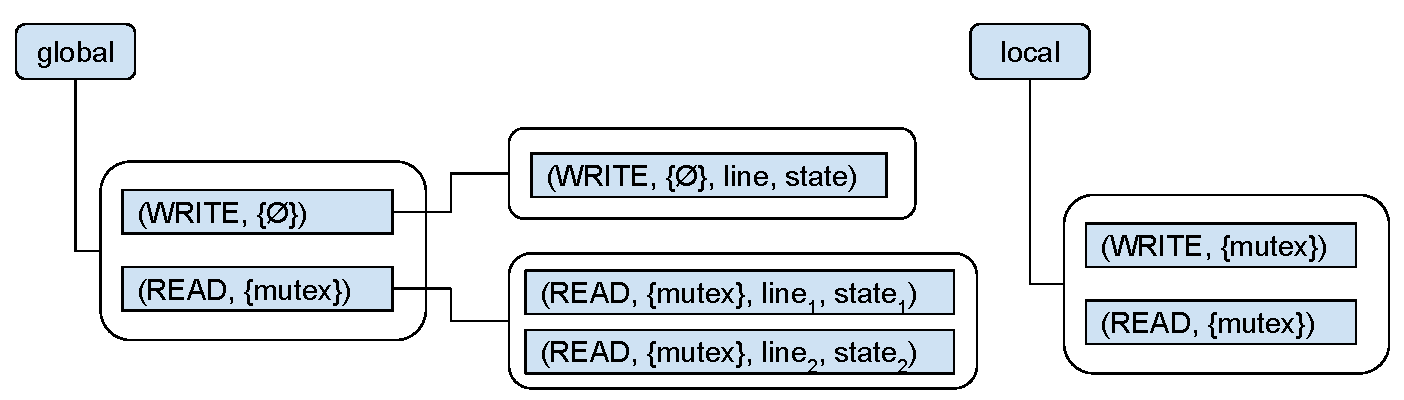
\includegraphics [scale=0.7] {GlobalContainer}
  \caption{Пример}
  \label{img:globalcontainer}
\end{figure}

Переменной $global$ соответствуют две точки использования: запись без использования примитивов синхронизации и чтение при захваченной mutex-блокировке. 
Причем второй точке использования соответствуют два реальных доступа, расположенных в разных строках исходного кода.

\section{Реализация уточнения} \label{sect_impl_refinement}

Уточнение абстракции по контрпримерам используется для того, чтобы исключить недостижимые пути из абстракции.
В классическом варианте CEGAR используется при решении задачи достижимости.
Когда найдено ошибочное состояние, начинается процесс уточнения: строится контрпример и проверяется, возможен ли такой сценарий в исходной программе. В случае, если такой путь является недостижимым из-за неточности абстракции, она уточняется таким образом, чтобы исключить такой путь из абстракции. 

При поиске состояний гонки дело усложняется тем, что ошибкой является не одно состояние, а пара. При этом каждый из путей сам по себе не является ошибкой.
Кроме того, обычно требуется обнаружить не первое состояние гонки в программе, а все потенциальные состояния гонки. 
Таким образом, возможны две вариации процедуры уточнения абстракции.

\begin{enumerate}
\item Уточнение производится в процессе анализа. При обнаружении пары состояний, составляющих состояние гонки, оба пути проверяются на достижимость. Если найденная ошибка подтверждается, она отмечается, как подтвержденная и анализ продолжается.
Этот вариант уточнения очень похож на классический вариант: при обнаружении ошибки абстракция уточняется до тех пор, пока ошибка либо не подтвердится, либо не опровергнется.
Такой подход обладает существенным недостатком: для корректного завершения анализа, требуется построить очень точную абстракцию. 
В случае, если анализируемый код содержит сотни тысяч строк кода, построение точной абстракции требует колоссального времени. 
Более эффективно в этом случае гибко задавать ограничения на ресурсы, чтобы иметь возможность завершить анализ в любой момент, хотя это и повлечет за собой некоторое снижение точности. 
Это позволяет сделать второй подход к уточнению.

\item Уточнение всех путей производится в тот момент, когда абстракция полностью построена. Все обнаруженные состояния гонки проверяются на истинность, и, в случае необходимости, абстракция перестраивается. 
Существенным недостатком этого подхода является большой объем лишней работы в том случае, если неточность абстракции затрагивает множество состояний гонки.
Тогда проверка каждой из них будет давать один и тот же результат.
Однако, возможно применение некоторых оптимизаций, которые позволяют сократить время на такую бесполезную работу. 
\end{enumerate}

Нужно отметить, что оба варианта уточнения способны исключать из абстракции только локально-недостижимые пути.
Пути, в которых неправильно моделируется взаимодействие потоков, не могут быть исключены из абстракции.

Для того, чтобы обеспечить гибкую настройку, процесс уточнения был разделен на функциональные блоки.
Каждый такой блок определяется тем, что он принимает себе на вход от предыдущего блока, и тем, что он выдает на выходе следующему.
Результатом работы каждого из абстрактных блоков является вердикт TRUE, означающий, что то, что передается на вход этому блоку, содержит состояния гонки, и вердикт FALSE, означающий, что состояние гонки обнаружить не удалось.
В последнем случае может быть выдана некоторая информация (precision), которая позволит более точно вычислить абстракцию на следующей итерации анализа.
В редких случаях возможен вердикт UNKNOWN, означающий, что однозначный ответ не может быть получен. 
В большинстве случаев такой вариант реализуется при некорректной работе сторонних компонентов, таких как решателей (англ. solver).

Цепочка блоков уточнения состоит из двух частей. Первая часть - служебная, которая используется для подготовки путей к уточнению и обработке полученной от других блоков информации. Эта часть содержит:

\begin{enumerate}

\item IdentifierIterator. Блок, принимающий на вход ReachedSet и последовательно перебирающий все возможные переменные, к которым был доступ.
Соответственно, следующий за ним блок обязан принимать на вход идентификатор переменной.
В случае, если хотя бы для одной переменной был получен вердикт FALSE, это означает, что уточнение прошло успешно, и необходимо перестроить абстракцию.
Если же для всех новых переменных вердикт был TRUE или UNKNOWN, это означает, что абстракция построена с достаточным уровнем точности, и все найденные состояния гонки являются истинными с точки зрения анализа.

Каждый вердикт FALSE сопровождается некоторой информацией о том, как следует уточнить абстракцию. Этот уровень точности сохраняется для каждой переменной отдельно, но при построении абстракции учитывается уровень точности, полученный для каждой из переменных. Однако, в случае если для  какой-либо переменной будет доказано, что она участвует в истинном состоянии гонки, то соответствующий этой переменной уровень точности сбрасывается. Это помогает не перестраивать слишком точную абстракцию тогда, когда это уже не нужно.

\item PointIterator. Блок, принимающий на вход идентификатор переменной и перебирающий все возможные пары $Point$, которые образуют состояние гонки. Каждая пара $Point$ проверяется следующим блоком. Если для некоторой пары $Point$ будет получен вердикт TRUE, это означает, что ни один следующий блок не смог найти противоречия, а значит, полученное состояние гонки истинное и в предыдущий блок возвращается результат TRUE. 

\item UsageIterator. Блок, принимающий на вход пару $Point$ и перебирающий все возможные пары $Usage$, соответствующие этой паре $Point$. Каждая пара $Usage$ проверяется следующим блоком. Если для некоторой пары $Usage$ будет получен вердикт TRUE, это означает, что ни один следующий блок не смог найти противоречия, а значит, полученное состояние гонки истинное и в предыдущий блок возвращается результат TRUE. 

\item PathIterator. Блок, принимающий на вход пару $Usage$ и перебирающий все возможные пары путей в абстракции, соответствующие этой паре $Usage$. Необходимо пояснить, почему в абстракции возможно несколько путей из начального состояния к тому состоянию, которое соответствует данному $Usage$. Дело в том, что из-за применении оптимизации BAM (подраздел~\ref{subsect_impl_bam}), тело функции будет проанализировано один раз, несмотря на то, что вызовов этой функции может быть несколько. В таких случаях для каждого вызова функции возможно несколько точек ее вызова. Если для некоторой пары путей будет получен вердикт TRUE, это означает, что ни один следующий блок не смог найти противоречия, а значит, полученное состояние гонки истинное и в предыдущий блок возвращается результат TRUE. 

\end{enumerate}

Далее идет вторая часть цепочки, которая занимается непосредственно проверкой корректности двух путей. Поэтому каждый из этих блоков принимает на вход и передает в следующий блок пару путей. Если текущий блок считает, что данная пара путей невозможна, в предыдущий блок возвращается результат FALSE.
Блоки уточнения из этой части не являются обязательными, поэтому допустима любая их комбинация.

\begin{enumerate}

\item PredicateRefiner. Основной инструмент для удаления из абстракции локально-недостижимых путей. 
Использует внутри себя классический PredicateRefiner, но дополнительно применяется некоторый набор оптимизаций для того, чтобы сократить время работы.
Например, при переборе всех возможных пар путей может часто возникать проверка отдельного пути на локальную-достижимость. 
Чтобы избежать лишних проверок, сохраняется результат каждого уточнения для пути, а также тот уровень точности, который нужен для исключения данного пути из абстракции.
Таким образом, если возникнет необходимость в уточнении этого же пути, не важно на этой же итерации уточнения или на любой из последующих, выдет использован сохраненный результат. 

\item Фильтр. Фильтром называется такой блок, который, выдавая результат FALSE, не предоставляет уровень точности для того, чтобы исключить полученный путь (пару путей) из абстракции. А это значит, что такая же пара путей будет получена и для следующей абстракции.
Такой фильтр, тем не менее, полезен тем, что при переборе всех подходящих путей может быть найдена такая пара, которая будет истинна.
Возможны различные варианты фильтров, например, такой, который отсеивает доступы к переменным, происходящим из специальных функций. 

\end{enumerate}

Последний блок в цепи является специальной заглушкой, которая всегда возвращает значение TRUE.

Оптимизированный вариант?

\section{Печать и визуализация} \label{sect_impl_visualiztion}

Визуализация найденных состояний гонок является важным моментом для практического применения инструмента.
Выдаваемой информации должно быть достаточно для того, чтобы разработчик смог понять, какие именно действия в программе могут привести к состоянию гонки.
Таким образом, основными требованиями к визуализации являются:

\begin{enumerate}

\item Отображение всех операторов, которые встречаются на пути к каждому из доступов, образующих состояние гонки

\item Отображение и визуальное выделение двух доступов, образующих состояние гонки

\item Отображение и визуальное выделение всех операций с примитивами синхронизации

\item Отображение справочной информации о состоянии гонки: множество захваченных примитивов синхронизации, тип и имя разделяемой переменной

\end{enumerate}

Основой формата вывода найденных состояний гонки является формат, описанный в .
Этот формат предполагает преставление пути к ошибке в виде графа.


Структура графа пути

%\newpage
%============================================================================================================================

\clearpage